%%%%%%%%%%%%%%%%%%%%%%%%%%%%%%%%%%%%%%%%%%%%%%%%%%%%%%%%%%%%%%%%%%% 
%                                                                 %
%                           INLEIDING                             %
%                                                                 %
%%%%%%%%%%%%%%%%%%%%%%%%%%%%%%%%%%%%%%%%%%%%%%%%%%%%%%%%%%%%%%%%%%% 


\chapter{Gedetailleerd ontwerpproces}

In hoofdstuk drie wordt een algemeen overzicht gegeven van de opbouw en werking van het programma. Er wordt echter niet dieper ingegaan op de onderliggende code van het programma. Dit hoofdstuk zal zich voornamelijk verdiepen in deze code, de structuur ervan en zullen de belangrijkste onderdelen ervan worden uitgelegd. Hiernaast zal er ook worden beschreven hoe de externe programma's moeten worden geïnstalleerd en hoe deze in het programma worden geïmplementeerd. 
\par
Om de gedachtengang achter het ontwerpproces makkelijker volgbaar te maken zal er in dit hoofdstuk vooral gebruikt gemaakt worden van een actieve schrijfwijze en de wetenschappelijke 'we'-vorm. De code zal worden uitgelegd aan de hand van listings die rechtstreeks uit de code van het programma komen. De volledige code kan worden teruggevonden in de bijlages van deze tekst.[Bijlage D] Het is mogelijk dat de lijnnummers die in de tekst voorkomen niet volledig overeenstemmen met de lijnnummers van het gehele bestand. Dit is te wijten aan het feit dat de code kan zijn aangepast na het afdrukken van deze tekst.
\par
In de eerste sectie zal de installatie van de externe programma's worden besproken. Eerst zal er gezien worden hoe de OpenBabelGUI moet geïnstalleerd worden. Hierna zal worden uitgelegd hoe PyCIFRW kan worden verkregen. De tweede sectie beschrijft aanvankelijk hoe er kan gecontroleerd worden of een bestand een CIF-bestand is. Vervolgens wordt er uitgelegd hoe OpenBabel en de CifFile module kunnen worden gebruikt in een Python script. Het tekenen van de celomkadering, atomen en bindingen met behulp van de bpy module wordt uitgelegd in de derde sectie van dit hoofdstuk. In de voorlaatste sectie wordt er verteld hoe een Blender add-on wordt opgebouwd en hoe deze ontworpen wordt. In de conclusie van dit hoofdstuk worden de belangrijkste punten van dit hoofdstuk nogmaals op een rijtje gezet.   

\section{Installatie van externe programma's}
Zoals in hoodstuk drie wordt beschreven gaan we gebruik maken van twee externe programma's die we zullen nodig zullen hebben om het programma uit te kunnen voeren, OpenBabel en PyCIFRW. Deze sectie legt uit hoe we deze kunnen installeren op een systeem. Hoewel deze in het geval van dit onderzoek met Windows 10 wordt gewerkt, werken deze software ook op oudere versies van Windows. Ons programma is gericht op besturingssysteemonafhankelijkheid, dit wil zeggen dat het ook op Linux en Apple moet werken. Het is echter mogelijk dat het installeren van deze externe programma's anders verloopt dan op Windows. De installatie van deze programma's zal in deze tekst echter enkel voor Windowssytemen worden uitgelegd.

\subsection{OpenBabel}  
De installatie van OpenBabel kan gevonden worden op hun webpagina: \url{http://openbabel.org/wiki/Category:Installation} en is gratis voor iedereen. Op deze pagina gaan we de OpenBabelGUI \textit{installer} downloaden, zie Figuur[4.1], let op dat de bit-versie met die van ons systeem overeenkomt. De download zou automatisch moeten starten. Ten slotte kunnen we de installatiewizard starten door het gedownloade bestand uit te voeren.
\par
Na het volgen van de installatiewizard zou de OpenBabel GUI moeten geïnstalleerd zijn op ons systeem, en kan het gebruikt worden in ons programma. Dit zal in het verdere verloop van dit hoofdstuk worden uitgelegd.

\subsection{PyCIFRW}
Om de PyCIFRW module op ons systeem te installeren hebben we nood aan een prompt waarop Pyhton3.7 kan worden uitgevoerd. Zo'n prompt kan verkregen worden door Anaconda te installeren en gebruik te maken van \textit{Anaconda prompt}. Vervolgens hebben we de Python pip installer nodig. Deze is automatisch aanwezig op Python3.7
\par 
Pip laat ons toe allerlei Python modules te installeren, waaronder de PyCIFRW module. Dit doen we met door volgend commando in te geven in het prompt:
\begin{lstlisting}[caption=,numbers=none,language= bash]
  pip install PyCifRW
\end{lstlisting}
Dit zorgt ervoor dat we nu toegang hebben tot de PyCIFRW module wanneer we Python uitvoeren en kan eenvoudig getest worden door Python op te starten en de volgende lijn code uit te voeren:
\begin{lstlisting}[caption=,numbers=none]
  import CifFile
\end{lstlisting}

Als er geen foutmelding wordt gegeven, wilt het zeggen dat de module correct is geïnstalleerd op onze Python installatie. 
\par
Doordat Blender een eigen Python installatie heeft, zal deze nog geen toegang hebben tot onze geïnstalleerde modules. Dit kunnen we oplossen door de map die de PyCIFRW module bevat te kopiëren naar de Python installatie van Blender. Deze map kunnen we vinden op plaats waar we Python hebben geïnstalleerd op ons systeem. In het geval dat Anaconda wordt gebruikt, vinden we deze module in de submap \textit{site-packages} van de installatiemap van Anaconda.(\textit{Anaconda3 \textgreater \textgreater{} Lib \textgreater \textgreater{} site-packages}).
Vervolgens moeten we deze map \textit{CifFile} kopiëren naar de Python installatie van Blender (\textit{blender-2.80.0-git.3c8c1841d72-windows64 \textgreater \textgreater{} 2.80 \textgreater \textgreater{} python \textgreater \textgreater{} lib \textgreater \textgreater{} site-packages}). 
\par
Een alternatieve methode om de PyCIFRW module werkende te krijgen op Blender, zonder nood te hebben aan een Python3.7 installatie, is door de \textit{CifFile} map rechtstreeks in de Pythoninstallatiemap van Blender te plaatsen. De \textit{CifFile} kan gedownload worden vanaf de GitHub pagina van deze thesis: \url{https://github.com/JarritB/Thesis}
  
\section{Inlezen van het bestand}

\subsection{Controleren van het bestand}
Vooraleer we het bestand kunnen omzetten met OpenBabel moeten we controleren of het gekozen bestand wel degelijk een CIF-bestand is, dit zou anders voor problemen kunnen zorgen in het verdere verloop van het programma.
\par
Om dit te controleren moeten we nakijken of ons bestand de extensie \textit{.cif} heeft, in sommige gevallen wordt de extensie met hoofdletters geschreven, hiermee dienen we dus ook rekening te houden. Omdat de bestandsnaam het volledige pad naar het bestand inhoudt, moeten we enkel de vier laatste tekens overhouden. Dit wordt gedaan op lijn 730 van Listing[4.1].
\par 
De variabele \textit{ext} zal nu enkel de laatste vier tekens van de filenaam bevatten. Bij een CIF-bestand zullen deze laatste vier altijd \textit{.cif} zijn, we moeten de variabele dus hiermee vergelijken. Door de \textit{.lower()} methode op te roepen op de extensie zal deze altijd naar kleine letters worden omgezet, en hoeven we dus geen rekening te houden met hoofdletters. In het geval dat de extensie niet gelijk is aan \textit{.cif} gaan we een foutboodschap weergeven in de terminal en gaan we in de \textit{user\_feedback} variabele ook een boodschap zetten die zal verschijnen op onze add-on, deze variabele wordt later verder uitgelegd. Omdat er een fout bestand is ingegeven zal het programma beëindigd worden met een \textit{return}, het heeft geen zin dit bestand proberen te tekenen. In listing[4.1] wordt de controle van het bestand gedaan.

\lstinputlisting[linerange={730-734},firstnumber=730,caption=Controle van de extensie]{listings/__init__.py}

\subsection{Uitvoeren van OpenBabel}
Nu we zeker weten dat we met een CIF-bestand te maken hebben kunnen we de inwendige symmetrie van het kristal wegwerken met OpenBabel. 
\par
Het oproepen van OpenBabel doen we met behulp van de \textit{subprocess} module van python. Wanneer we deze module oproepen zal er een nieuw process worden gestart, die in ons geval OpenBabel zal uitvoeren.
\par
Voor we de \textit{subprocess} module kunnen oproepen in ons script moeten we  deze importeren met de lijn code in Listing[4.2]

\lstinputlisting[linerange={13-13},firstnumber=13,caption=Importeren van de subprocess module]{listings/__init__.py}

Vooraleer we OpenBabel gaan oproepen gaan we controleren of OpenBabel wel geïnstalleerd is op ons systeem. Dit wordt gedaan met een \textit{try-except} blok, zie Listing[4.3], welke gaat proberen de code in het \textit{try} gedeelte uit te voeren. Als dit niet lukt zal het programma in plaats daarvan het \textit{except} gedeelte uitvoeren. Bij een correcte installatie van OpenBabel zal de \textit{obabel\_fill\_unit\_cell} functie worden uitgevoerd, zie lijn 739 van Listing[4.3].
\par
In het geval dat OpenBabel niet kan worden opgeroepen gaan we een foutboodschap weergeven in de terminal en in de \textit{user\_feedback} variabele en zal ons programma verder werken met het ingegeven CIF-bestand. Hoewel het kristal niet kan geconverteerd worden, zullen we toch een deel van het kristal kunnen tekenen. In sommige gevallen heeft het ingegeven kristal geen inwendige symmetrie, en is er geen nood aan OpenBabel om het kristal te kunnen visualiseren.

\lstinputlisting[linerange={736-744},firstnumber=736,caption=Controle van de OpenBabel installatie]{listings/__init__.py}
\par	
De functie \textit{obabel\_fill\_unit\_cell} heeft het pad naar het ingevoerde CIF-bestand en de naam van het geconverteerde CIF-bestand als argumenten en bestaat uit slechts één lijn code. Op deze lijn roepen we de \textit{run} methode op de \textit{subprocess} module op, deze heeft als argument een \textit{string} waarin het uit te voeren commando staat zoals het in een prompt zou worden uitgevoerd. Het commando waarmee we OpenBabel uitvoeren, bestaat uit volgende parameters:
\begin{itemize}
\item obabel: roept OpenBabel op
\item -icif: type van het invoerbestand, wordt gevolgd door de bestandsnaam
\item -ocif: type van het uitvoerbestand
\item -O: gevolgd door naam van het uitvoerbestand
\item --fillUC: selecteert de mode waarin de symmetrie zal worden omgezet
\item keepconnect: parameter van de fillUC mode, tekent ook atomen buiten de eenheidscel
\end{itemize}
In onze code ziet het er dan als volgt uit:
\lstinputlisting[linerange={675-675},firstnumber=675,caption=Uitvoeren van OpenBabel]{listings/__init__.py}

\subsection{Zelf een parser ontwerpen}
In de vierde sectie van hoofdstuk twee werd er reeds aangehaald wat er allemaal komt kijken bij het ontwerpen van een parser. Het is gelukt een programma[Bijlage C] te ontwerpen dat alle CIF-bestanden kan inlezen die te vinden zijn op de kristallografische databank van het IZA.\citep*{IZA1} Het parsen van deze bestanden lukte echter enkel omdat deze allemaal dezelfde tekststructuur bezitten. Bestanden uit databanken die werken met een andere structuur kunnen mogelijks verkeerd worden geïnterpreteerd waardoor de parser zijn nut verliest. Het is mogelijk de code van de parser aan te passen zodat, ongeacht de structuur van het CIF-bestand, een juiste interpretatie van de data kan worden gedaan. Dit vergt echter veel tijd en zal, gezien er reeds werkende CIF-parsers bestaan, niet verder worden onderzocht.



\subsection{Parsen met PyCifRW}
Het geconverteerde bestand parsen gaan we doen met behulp van de CifFile module van PyCIFRW. Om toegang te krijgen tot deze module moeten we deze eerst importeren in onze code, zie Listing[4.5]. Omdat er hier een fout wordt gegeven als de module niet geïnstalleerd is, moeten we deze import omsluiten met een \textit{try-except} blok. Als de module niet kan geïmporteerd worden gaan we een variabele aanzetten zodat het programma later weet dat het een foutmelding moet geven aan de gebruiker.

\lstinputlisting[linerange={16-21},firstnumber=16,caption=Importeren van de CifFile module]{listings/__init__.py}

Met de CifFile module kunnen we vervolgens een \textit{CifFile} object aanmaken. Door de bestandsnaam mee te geven als argument zal de CifFile module automatisch het bestand parsen en de data opslaan in het object, dit wordt gedaan op lijnen 740 en 744 van Listing[4.3]. Naast het \textit{CifFile} object maken we ook een object van de \textit{Crysdata} klasse aan. Deze klasse heeft een initialisatiemethode die zal worden uitgevoerd zodra een object ervan wordt aangemaakt, zie Listing[4.6]. In deze methode gaan we de attributen van de klasse bepalen. Enkele interessante attributen van deze klasse zijn:

\begin{itemize}
\item start: start een soort van timer op, zo kan de loopduur van het programma worden nagekeken
\item cell: een object van de \textit{Cell} klasse, bevat de roosterparameters
\item atoms: een lijst van objecten van de klasse \textit{Atom}, alle atomen van het eenheidskristal
\item pos: een lijst met alle inwendige symmetrieën van het kristal, deze wordt voorlopig niet gebruikt
\item ftoc: de fractionele naar orthogonale conversiematrix, deze wordt berekend aan de hand van de roosterparameters
\end{itemize}

In Listing[2.7] van hoofstuk twee werden de voornaamste functies van de CifFile module reeds beschreven. In hoofdstuk drie zagen we ook dat zo een \textit{CifFile} object kan gezien worden als een dictionary. Alleenstaande gegevens in het datablok van het CIF-bestand, zoals de roosterparameters, kunnen we eenvoudig opvragen met de correcte sleutels. Dit doen we om een object van de klasse \textit{Cell} aan te maken, zie Listing[4.6].

\lstinputlisting[linerange={576-583},firstnumber=576,caption=Initialisatiemethode van de klasse Cell]{listings/__init__.py}

Het toekennen van het object \textit{atoms} doen we met een aparte functie. In deze functie gaan we nieuwe \textit{Atom} objecten aanmaken, deze invullen met data door het lusblok met atom in \textit{CifFile} object te doorlopen en deze in een lijst plaatsen. Dit wordt gedaan in Listing[4.7] 

\lstinputlisting[linerange={639-659},firstnumber=639,caption=Functie die een lijst van atomen aanmaakt]{listings/__init__.py}

In de conversie die OpenBabel doet krijgen de atomen dezelfde ID toegekend als het atoom waarvan de symmetriepositie is berekend, om dit op te lossen dienen we een lijst bij te houden met de ID's van de atomen die we al hebben aangemaakt en een teller bij te houden van het aantal van atomen met deze ID. Als er een atoom met hetzelfde ID voorkomt, zal er aan dit ID een nummer worden toegevoegd en gaan we de teller met één verhogen. Op deze manier zijn we zeker dat elk atoom een eigen ID heeft waarmee het later kan worden aangesproken.    

\section{Tekenen in Blender}

\subsection{Programmeren met de Blender API}
Tot nu toe zijn we in staat een CIF-bestand te converteren met OpenBabel, vervolgens te parsen met PyCIFRW en een \textit{Crysdata} object te creëren waarin de kristalinformatie staat. De volgende stap is het visualiseren van deze data in de Blender omgeving. Hiervoor gaan we gebruikmaken van de Blender API en meer specifiek, de bpy module die de Blender API aanbiedt. 
\par
Zoals met elke module die we tot nu toe gebruikt hebben, moeten we de bpy module eerst importeren. Omdat deze module niet bereikbaar is buiten de Blender omgeving gaan we weer gebruikmaken van een \textit{try-except} blok, welke zal proberen de module te importeren. Als dit lukt gaan we een variabele aanzetten zodat ons programma weet dat het mogelijk is deze module te gebruiken, zoniet zal het een foutboodschap geven, maar zal alles anders wel worden gedaan zodat het programma kan getest worden buiten de Blender omgeving.
\par
Het tekenen van het kristal is een methode van de \textit{Crysdata} klasse, deze zal stap voor stap functies aanroepen waarin bepaalde onderdelen van het kristal worden getekend. Wanneer de gebruiker zich niet in de Blender omgeving bevindt zal ons programma deze methode niet oproepen. 

\subsection{Tekenen van de omkadering}

Het tekenen van de omkadering van de eenheidscel is het eerste wat er zal gebeuren. Omdat het tekenen van de omkadering een optie is die de gebruiker kan aanzetten, gaan we eerst controleren of deze stap wel moet gebeuren, anders wordt deze overgeslagen.
\par
De \textit{drawCell} methode is er een van de \textit{Crysdata} zelf. Deze methode zal met behulp van de conversiematrix en de roosterparameters, welke te vinden zijn als attributen van het \textit{cell} object, eerst kleine bollen tekenen op de hoekpunten van de eenheidscel. Dit wordt gedaan in Listing[4.8]. 

\lstinputlisting[linerange={451-459},firstnumber=451,caption=Tekenen en kleuren van de hoekpunten van de eenheidscel]{listings/__init__.py}

Dit is het ideale moment om enkele, in ons programma vaak voorkomende, functies van de bpy module uit te leggen. Het aanmaken van nieuwe vormen wordt gedaan met de \textit{bpy.ops.mesh} functie. Op lijn 454 van Listing[4.8] roepen we deze functie op om een \textit{primitive\_uv\_sphere} te tekenen. Deze vorm is een type van bol. In de volgende lijnen gaan we onze net aangemaakte bol als actief object zetten zodat we aan dit object een nieuw materiaal kunnen toekennen. Door een vorm een materiaal toe te kennen kunnen we een kleur geven aan het materiaal, en aan onze bol. Kleuren worden in Blender aan de hand van RBG-waarden bepaalt, deze waarden worden in de vorm van een lijst gegeven waarin het niveau van elke kleur (rood, groen, blauw) met een getal tussen nul en één wordt voorgesteld. In het geval van onze bol kiezen gebruiken we de waarden [0,0,0], welke zwart voorstellen.
\par
Nu we onze hoekpunten hebben bepaald, en getekend, moeten we de ribben van onze omkadering tekenen. Dit gaan we doen door cilinders te tekenen tussen de hoekpunten van de eenheidscel. Door een lijst bij te houden waarin de bollen worden opgeslagen wanneer ze worden aangemaakt, zie lijn 456 van Listing[4.8], kunnen de hoekpunten worden verkregen. Omdat we niet tussen alle hoekpunten een lijn willen tekenen, dit zou namelijk ook de diagonalen tekenen, gaan we specifiëren tussen dewelke we een lijn willen tekenen. Door de hoekpunten in een lijst bij te houden zijn deze in essentie genummerd. We gaan twee lijsten aanmaken die elk één nummer bevatten van de koppels van hoekpunten die we willen verbinden. Door gebruik te maken van de \textit{zip} functie van Python kunnen we deze lijsten samennemen en er twee variabelen tegelijk over itereren. Deze twee variabelen stellen telkens het paar van hoekpunten voor waartussen we een cilinder gaan tekenen. Vervolgens gaan we aan de hand van de locaties van de hoekpunten de afstand ertussen berekenen, dit wordt de lengte van onze cilinder. Het tekenen van de cilinder wordt op een gelijkaardige manier gedaan als we eerder hebben gedaan bij het tekenen van de hoekpunten. De cilinder zal vertrekken op de plaats van het eerste hoekpunt en met behulp van enkele goniometrische berekeningen kunnen we de cilinder zo roteren dat het uiteinde overeenkomt met het andere hoekpunt.
\par

\lstinputlisting[linerange={464-470},firstnumber=464,caption=Samennemen van alle objecten in een vorm]{listings/__init__.py}

Ook de ribben van de cel gaan we bijhouden in een lijst. Op deze manier kunnen we na het tekenen van de ribben alle objecten uit de lijsten van hoekpunten en ribben selecteren en samenvoegen in één object. Dit wordt gedaan in Listing[4.9].     

\subsection{Tekenen van atomen}

Het tekenen van de atomen doen we met de \textit{drawAtoms} methode van de \textit{Crysdata} klasse. Deze methode zal de lijst met atomen aflopen en op elk element van deze lijst de \textit{drawObj} methode oproepen. De \textit{drawObj} methode is een methode van de \textit{Atom} klasse en wordt weergegeven in Listing[4.10] 

\lstinputlisting[linerange={609-621},firstnumber=609,caption=De tekenmethode van de klasse \textit{Atom}]{listings/__init__.py}

Om elk element een eigen grootte en kleur te geven maken we gebruik van twee dictionaries, het is mogelijk deze samen te nemen in één dictionary om minder geheugen te gebruiken, dit maakt het echter minder overzichtelijk voor de gebuiker. Omdat deze dictionaries meer dan 90 elementen bevatten, worden deze niet rechtstreeks in de code opgenomen, maar zullen we ze in een extern bestand opslaan. Op deze manier hoeft een gebruiker het bronbestand van het programma niet aan te passen, wanneer deze de dictionaries wil bewerken. Deze externe dictionaries kunnen worden gevonden als bijlagen van deze tekst.[Bijlage E \& F] Het inlezen van een dictionary vanuit een extern bestand wordt gedaan met behulp van de \textit{eval} functie. Deze functie heeft als argument een string, welke \textit{eval} als Python code zal interpreteren. Het inlezen van een externe dictionary wordt gedaan in Listing[4.11]. 
  
\lstinputlisting[linerange={88-89},firstnumber=88,caption=Inlezen van een dictionary vanuit een extern bestand]{listings/__init__.py}

De tekenmethode van het atoom zal, met het symbool van het element als sleutel, de straal van het atoom uit de \textit{sizedic} dictionary halen. Om de positie van het atoom te bepalen, wordt de conversiematrix gebruikt. Deze zal de fractionele coördinaten, die attributen zijn van het \textit{Atom} object, omzetten naar hun orthogonale waarden. Dan tekenen we een bol met de eerder bepaalde straal op die plaats. De straal hangt ook af van de stijl waarin het kristal zal worden getekend. Bij de \textit{STICK AND BALL} stijl zal de straal worden gehalveerd, zodat de bindingen zichtbaar worden. Bij de \textit{STICK} tekenstijl zal de straal zo klein zijn dat enkel de bindingen nog zichtbaar zijn. De argumenten \textit{segments} en \textit{ring\_count} op lijn 611 van Listing[4.10] bepalen uit hoeveel vlakken de bol bestaat, bij een lage waarde zal de bol eerder hoekig zijn. De gebruiker kan het aantal segmenten kiezen waarmee het aan de hand van een dictionary wordt ingevuld.
\par
Op lijn 612 van Listing[4.10] kennen we de getekende bol een naam toe, via deze naam kunnen we onze bol later terugvinden in de lijst van getekende objecten. Hierna gaan we onze bol een materiaal en een kleur toekennen. De kleur wordt bepaald door de waarde die terug te vinden is in \textit{colordic}, dit is de dictionary waarin de kleuren van de elementen wordt gegeven. Als het kristal in de \textit{STICK} tekenstijl wordt getekend zullen de bollen steeds een witte kleur krijgen toegekend.
\par

\subsection{Tekenen van bindingen}    

De gebruiker heeft de mogelijkheid om bindingen tussen atomen te laten tekenen, in de {STICK} tekenstijl zullen deze bindingen steeds worden getekend. Het tekenen van bindingen wordt gedaan in de \textit{drawBonds} methode van de \textit{Crysdata} klasse. Deze methode zal in eerste instantie een béziercirkel tekenen en het de naam \textit{bez} toekennen, deze cirkel zal gebruikt worden als vorm waarmee een \textit{bevel} zal worden gedaan, later hier meer over. Vervolgens gaan we de lijst van atomen doorlopen per element deze lijst nogmaals doorlopen, op deze manier kunnen we de afstand tussen elk element berekenen. Voor we deze afstand gaan berekenen gaan we eerst twee testen doen om te voorkomen dat het programma dubbel werk doet. Eerst gaan we na of de twee atomen dezelfde zijn, in dit geval zou het nutteloos zijn een binding te tekenen. De tweede test gaat in de lijst van getekende objecten kijken of er al een binding bestaat tussen deze twee atomen, zo vermijden we dat we de binding tweemaal tekenen. De \textit{bpy.data} module van de Blender API geeft ons toegang tot alle interne data van de Blender omgeving. Door \textit{bpy.data/objects} op te roepen krijgen we een dictionary waarin alle objecten kunnen worden opgeroepen aan de hand van hun ID. Doordat we onze bindingen een naam geven gebaseerd op de atomen die gebonden worden hebben we zo een manier om reeds bestaande bindingen te vinden.
\par
De gebruiker kan zelf de maximale afstand instellen die tussen twee atomen mag zijn om er een binding tussen te tekenen. De afstand tussen twee atomen gaan we berekenen met de formule:
\[ d = \sqrt{(x_{a1}-x_{a2})^2+(y_{a1}-y_{a2})^2+(z_{a1}-z_{a2})^2}\]   
Met a1 de orthogonale coördinaten van het eerste atoom en a2 die van het tweede.
\par
Enkel wanneer deze afstand kleiner is dan diegene die de gebruiker kiest, moeten we een binding tekenen tussen de atomen. Hiervoor wordt de \textit{makeBond} methode opgeroepen met de twee te binden atomen als argument. Deze methode gaat eerst met de \textit{bpy.data} module de twee bollen zoeken die de atomen voorstellen. Deze twee objecten zullen dienen als argumenten van de volgende methode die we gaan oproepen, \textit{hookCurve}. In deze methode worden enkele, eerder abstracte, methodes van de bpy module gebruikt, daarom zal deze stap voor stap worden doorlopen.

\lstinputlisting[linerange={531-532},firstnumber=531,caption=]{listings/__init__.py}

Eerst wordt er een \textit{curve}, of kromme,  aangemaakt. Deze krijgt de naam \textit{link} en het type \textit{CURVE} toegewezen. We zeggen ook meteen dat de kromme driedimensionaal is, dit zorgt anders later voor problemen. Merk op dat we onze nieuwe kromme niet in de lijst van objecten aanmaken, we creëren in feite een nieuwe vorm die we later als object kunnen aanmaken. 

\lstinputlisting[linerange={533-533},firstnumber=533,caption=]{listings/__init__.py}
Vervolgens gaan we nieuwe splines toevoegen aan de kromme. Splines zijn in feite lijnsegmenten waarmee een kromme kan worden voorgesteld, in ons geval gaan we werken met slechts één spline die van het type \textit{bézier} is. Dit zal van onze kromme een bézierkromme maken. Een bézierkromme is een manier waarop lijnen wiskundig kunnen worden voorgesteld aan de hand van twee of meer punten, die de graad van de 	bézierkromme bepalen volgens: $graad = n - 1$. Figuur[4.1] geeft een voorbeeld van een kromme die bepaald wordt door vier punten. Omdat we in ons geval enkel met rechte lijnstukken gaan werken volstaat een bézierkromme van de eerste graad en hoeven we niet dieper in te gaan op de wiskundige berekening van de vorm.

\begin{figure}[H]
\begin{center}
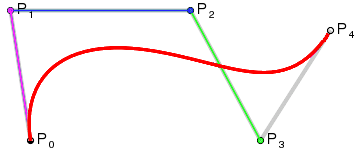
\includegraphics[]{bezier.png}
\caption{Voorbeeld van een bézierkromme met graad 3 \citep*{BEZ1}}
\end{center}
\end{figure}

Momenteel bestaat onze spline uit één bézierpunt, we moeten er dus nog één toevoegen om een lijn te bekomen.

\lstinputlisting[linerange={535-537},firstnumber=535,caption=]{listings/__init__.py}

We kennen onze bézierpunten toe aan variabelen zodat deze later makkelijk kunnen worden opgeroepen.

\lstinputlisting[linerange={544-548},firstnumber=544,caption=]{listings/__init__.py}

Nu gaan we van onze kromme een object maken in de Blender omgeving. Aan zo een object kunnen we vervolgens \textit{modifiers} toevoegen. In ons geval gaan we gebruik maken van de \textit{hook modifier}, deze zal het object vasthechten aan een ander object. We maken een nieuwe \textit{hook modifier} aan en noemen deze \textit{alpha}. We hechten deze aan \textit{o1}, het eerste atoom, vast. Dit doen we vervolgens nogmaals voor \textit{o2}, het tweede atoom, en geven deze de naam \textit{beta}. Onze 'haken' hangen nu vast aan onze atomen, maar nog niet aan onze kromme.

\lstinputlisting[linerange={550-553},firstnumber=550,caption=]{listings/__init__.py}  

We gaan eerst onze kromme toevoegen aan onze collectie, hierna kunnen we onze kromme als actief object selecteren. Dit is nodig omdat we in de volgende lijn de tekenmode van Blender gaan veranderen naar de \textit{EDIT} mode. In deze mode worden alle hoekpunten van het actieve object zichtbaar en kan de geometrie van deze in meer detail worden aangepast. We zullen de \textit{EDIT} mode gebruiken zodat we in de volgende stap de twee bézierpunten van onze kromme apart kunnen selecteren. 

\lstinputlisting[linerange={560-562},firstnumber=560,caption=]{listings/__init__.py}

Herinner dat we eerder onze twee bézierpunten aan de variabelen \textit{p0} en \textit{p1} hebben toegekend. Deze variabelen kunnen we nu gebruiken om de punten op een eenvoudige wijze te (de)selecteren. Eerst gaan we \textit{p0} selecteren en \textit{p1} deselecteren. Dan kunnen we \textit{p0} vasthangen aan de eerste \textit{hook modifier} die we \textit{alpha} hebben genoemd. Dit gaan we herhalen voor \textit{p2} en \textit{beta}. Figuur[4.2] toont een overzicht van welke \textit{modifier} welke objecten vasthecht.  

\begin{figure}[h]
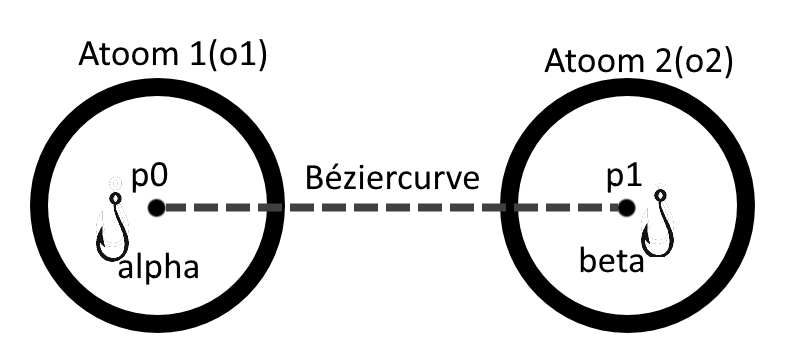
\includegraphics[scale=0.4]{hookmod.png}
\begin{tabular}{lll}
\hline
\multicolumn{1}{|l|}{Modifier} & \multicolumn{1}{l|}{Object} & \multicolumn{1}{l|}{Bézierpunt} \\ \hline
alpha                          & o1                          & p0                              \\
beta                           & o2                          & p1                             
\end{tabular}
\caption{Overzicht van de \textit{hook modifier}}
\end{figure}

Het vasthechten van objecten zal steeds gebeuren in het originepunt van een object. Als dit punt niet wordt verplaatst zal het zich steeds in het midden van een object bevinden. Hierdoor zal de kromme steeds gebonden zijn aan het midden van de bollen.
\par
Hoewel we nu een kromme hebben getekend tussen onze atomen, gaan we deze nog niet kunnen zien. Omdat een kromme geen volume heeft, zal deze niet zichtbaar zijn op het scherm. Er is nog één laatste stap die we moeten volgen om onze bindingen te tekenen, een \textit{bevel}.

\lstinputlisting[linerange={519-519},firstnumber=519,caption=]{listings/__init__.py}

In het begin van deze sectie hebben we een béziercirkel, \textit{bez} getekend. Deze gaat nu van pas komen, we gaan namelijk een \textit{bevel} uitvoeren. Een \textit{bevel}, ook wel een \textit{sweep} genoemd, een term uit de wereld van het computertekenen die ruwweg betekent: een driedimensionale vorm creëren door een bepaalde vorm over een pad te extruderen. Op Figuur[3.4] wordt een \textit{bevel} gedaan van een cirkel over een recht lijnstuk waardoor een cilinder wordt gecreëerd. In realiteit zal er in Blender geen nieuw object worden aangemaakt bij een \textit{bevel}, het is een eigenschap van de kromme die het zijn driedimensionale structuur geeft.  

\begin{figure}[H]
\begin{center}
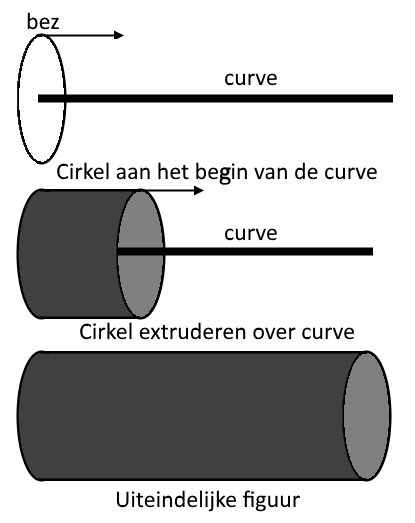
\includegraphics[scale=0.6]{bevel.png}
\end{center}
\caption{Eenvoudig voorbeeld van een \textit{bevel}}
\end{figure}

Nu we de binding succesvol kunnen tekenen hoeven we ze enkel nog een naam en kleur te geven. Voor de kleur van de bindingen gebruiken we wit, zo zijn ze duidelijk zichtbaar in het kristal.

\section{Ontwerpen van een Blender add-on}

\subsection{Add-on header}

In onze code schrijven we een header, als een dictionary met de naam \textit{bl\_info}, waarin we de nodige informatie over de add-on zetten, zie Listing[4.12]. Figuur[4.4] toont aan hoe onze add-on wordt afgebeeld in de \textit{user\_preferences} onder het \textit{add-on} tabblad. We merken op dat beide het \textit{name} veld en het \textit{category} veld van de header gebruikt wordt om de add-on initieel weer te geven. De andere velden worden pas zichtbaar als er op het pijltje linksboven wordt gedrukt. We moeten dus de naam en categorie van onze add-on dusdanig kiezen dat een gebruiker meteen weet waarvoor ze dient. 

\lstinputlisting[linerange={103-110},firstnumber=103,caption=De bl\_info header van onze add-on]{listings/__init__.py}

Als naam is er voor \textit{Crystallographic Drawing Tool for Blender}, afgekort naar \textit{CDTB}, gekozen. De catergorie spreekt voor zichzelf, en in de beschrijving van de add-on wordt er vermeld dat het programma met CIF-bestanden werkt. De locatie van de add-on is het \textit{View3D} venster, omdat hier het kristal zal  getekend worden.

\begin{figure}[H]
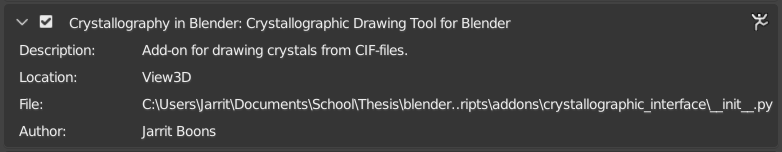
\includegraphics[width=\textwidth]{add-on.png}
\caption{Onze add-on afgebeeld in de \textit{user\_preferences}}
\end{figure}

\subsection{Schrijven van operatoren}

Zoals in hoofdstuk drie wordt beschreven gaan we twee operatorklassen maken. Met de eerste operator willen we een bestandsbrowser openen waarin we het CIF-bestand kunnen selecteren dat we willen tekenen. 

\lstinputlisting[linerange={129-132},firstnumber=129,caption=De invoke methode van de eerste operator]{listings/__init__.py}

Deze klasse geven we een methode \textit{invoke}, zie Listing[4.13], deze zal ervoor zorgen dat zodra de operator wordt uigevoerd er een filebrowser opent, met de \textit{return} op lijn 132 zorgen we ervoor dat deze operator blijft lopen zolang de bestandsbrowser is geopend. Wanneer we een bestand selecteren, zal de \textit{execute} methode het pad naar het bestand aan een globale variabele toekennen, zodat deze leesbaar is vanuit heel het programma, en stopt de operator.
\par 
Bij het maken van de tweede operatorklasse komt iets meer werk kijken. Eerst moeten we alle attributen aanmaken die we later in het paneel willen kunnen aanpassen. Dit doen we in de \textit{register} methode, met behulp van de \textit{bpy.props} module. Met deze module gaan we de attributen aanmaken die moeten geïnterpreteerd worden door het paneel. Een voorbeeld van de creatie van zo een attribuut zien we in Listing[4.14].      

\lstinputlisting[linerange={210-217},firstnumber=210,caption=Het initialiseren van het \textit{bond\_distance} attribuut ]{listings/__init__.py}

Met het attribuut in Listing[4.14] zal de gebruiker de maximale bindingsafstand kunnen kiezen, omdat deze afstand een kommagetal mag zijn gebruiken we een \textit{FloatProperty}. Deze functie krijgt enkele argumenten meegegeven:

\begin{itemize}
\item name: de naam die in het paneel zal worden weergegeven
\item description: een beschrijving van het attribuut welke te zien is als de cursor over het attribuut hangt
\item default: de waarde die het attribuut heeft wanneer de add-on wordt ingeladen
\item min/max: de uiterste waarde die de gebruiker kan invullen
\item precision: het aantal getallen na de komma dat het attribuut kan hebben
\end{itemize}  

Wanneer het attribuut een \textit{IntProperty} of een \textit{BoolProperty} is zullen sommige van deze parameters, zoals de precisie, niet van toepassing zijn. Enumeraties werden in hoofdstuk drie reeds besproken. Attributen van het type \textit{EnumProperty} kunnen enkel de waarde hebben van een van de elementen van de enumeratie die wordt meegegeven als parameter \textit{item}.
\par
De \textit{execute} methode van de tweede operator gaat aanvankelijk, net zoals de eerste operator, zijn attributen toekennen aan globale variabelen zodat ze leesbaar zijn vanuit heel het programma. Hierna roept de operator de functie \textit(drawCrystal) op, en zal de code die we bespraken in sectie twee en drie  worden uitgevoerd.  

\subsection{Creëren van de user interface}
Als link tussen onze add-on en de gebruiker gaan we gebruik maken van de \textit{Panel} klasse van Blender. Bij aanmaken van een paneel moeten we deze eerst enkele belangrijke attributen toekennen, zie Listing[4.15].
 
\lstinputlisting[linerange={274-279},firstnumber=274,caption= Enkele belangrijke attributen van de paneelklasse ]{listings/__init__.py}

Met deze attributen bepalen we hoe en waar we de add-on willen weergeven, en welke naam er bovenaan het paneel staat. In de \textit{draw} methode gaan we de layout van het paneel personaliseren. Om de add-on gebruiksvriendelijk te houden gaan we de opmaak van het paneel beperken tot enkele vakken, symbolen en gaan we geen specifieke kleuren toekennen.
\par
De paneelklasse heeft een attribuut \textit{layout} waarop we verschillende methodes kunnen oproepen. Telkens we zo een methode oproepen wordt er een onderdeel toegevoegd aan het paneel. Deze methodes kunnen we ook oproepen op de onderdelen van het paneel, zo kunnen we ze verder onderverdelen. Listing[4.16] toont een deel van de \textit{draw} methode waarin we het paneel opbouwen door een reeks van deze methodes in een bepaalde volgorde op te roepen. Het blok code van Listing[4.16] komt overeen met het deel van paneel dat zich in de rode kader bevindt op Figuur[4.5]. Op deze manier kunnen we de code stap voor stap vergelijken met ons uiteindelijke paneel.   

\lstinputlisting[linerange={294-304},firstnumber=294,caption= Het opbouwen van een paneel]{listings/__init__.py}

Op de eerste lijn van Listing[4.16] maken we een vak aan met de \textit{box} methode, dit zal een kader tekenen rond alles wat zich in dit vak bevindt. Hierna maken we een rij aan in het vak door de \textit{row} methode op de variabele \textit{box} op te roepen. Deze rij splitsen we op en verdelen deze in twee kolommen, waarvan de linker slechts 7.5\% van de volledige breedte van het paneel is. Op de linkerkolom roepen we de methode \textit{operator} op, lijn 299. Hiermee plaatsen we een drukknop die de operator uitvoert waarmee we een bestand kunnen inlezen. We zetten geen tekst op de drukknop maar gebruiken het icoon van een map, deze heeft 108 als ID. In de rechterkolom plaatsen we een label waarop de globale variabele van het pad naar het bestand wordt geschreven. Omdat het volledige pad niet in het paneel past, laten we alle tekens voor het laatste scheidingsteken vallen zodat we enkel de bestandsnaam en extensie overhouden. Dit is het laatste dat we toevoegen in dit vak van het paneel.
\par
\begin{figure}[H]
\begin{center}
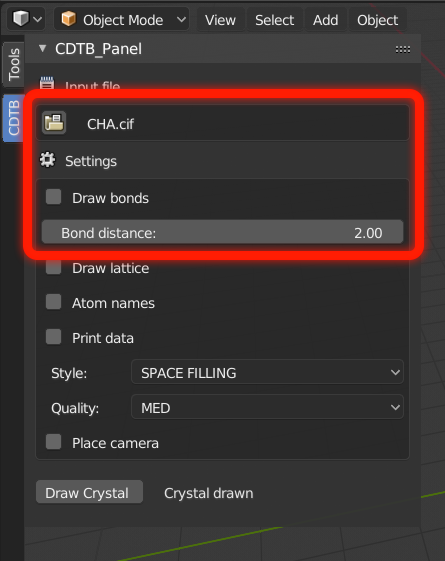
\includegraphics[scale=0.6]{opbouw.png}
\caption{Het paneel (onderdelen uit Listing[4.16] in rode kader)}
\end{center}
\end{figure}

Vooraleer we een nieuw vak gaan aanmaken, voegen we een label toe en geven dit zowel de naam \textit{settings} als een icoon. Dit label is de titel van het volgende vak, wat niet alleen esthetisch aangenaam is, maar ook overzichtelijk is voor de gebruiker.
\par 
Hierna maken we een nieuw vak aan waarin we alle tekenopties gaan geven. Deze opties zijn de attributen van de tweede operatorklasse en geven we weer door de \textit{prop} methode op the roepen op het vak, en de naam van het attribuut als parameter mee te geven. Een \textit{BoolProp} zoals \textit{draw\_bonds} zal worden weergegeven als een selectievakje, en \textit{bond\_distance}, dewelke een \textit{FloatProp} is, zal in ons paneel als een invoerveld en schuifbalk worden weergegeven.
     
  
\section{Conclusie}

In dit hoofdstuk hebben we eerst bekeken hoe we de OpenBabelGUI moeten installeren op een Windowssysteem, zodat we dit in ons programma kunnen oproepen als subprocess. Hierna hebben we ons verdiept in de installatie van de CifFile module van PyCIFRW. Deze kunnen we installeren op een systeem aan de hand van een Python3.7 installatie en de pip installer. Deze stap kunnen we overslaan door de map met de CifFile module meteen in de Pythoninstallatie van Blender te plaatsen.
\par
Na dieper in te gaan op de installatie van deze externe programma's hebben we de onderliggende code van ons programma onder de loep genomen en de werking van enkele belangrijke functies overlopen. We zagen onder andere hoe we controleren of een bestand een CIF-bestand is en hoe we met de subprocess module van Python OpenBabel als extern process kunnen oproepen om het CIF-bestand te converteren naar één zonder inwendige symmetrie. 
\par
We hebben kort aangehaald hoe het is om zelf een CIF-parser te ontwerpen en merkten dat dit, hoewel doenbaar, erg veel werk is. Aangezien dit niet de essentie van het onderzoek is, zijn we hier niet verder op ingegaan. 
\par 
Vervolgens hebben we bekeken hoe we met behulp van de CifFile module van PyCIFRW CIF-bestanden kunnen parsen. We hebben een voorbeeld bekeken waarin we de roosterparameters van een kristal aan de variabelen van de Cell toekennen, en hoe de lijst van atomen kan verkregen worden door het lusblok van een CIF-bestand te doorlopen. Omdat OpenBabel nieuwe atomen geen eigen ID geeft, hebben we zelf een manier gevonden die met een lijst en een teller elk atoom van het kristal een unieke ID geeft.
\par 
Het tekenen in Blender doen we met behulp van de bpy module die de Blender API aanbiedt. Deze module hebben we onder andere gebruikt om de omkadering van het eenheidskristal te tekenen. Dit doen we door eerst de hoekpunten te tekenen als bollen en deze nadien met elkaar te verbinden met behulp van cilinders. We zagen ook hoe we een materiaal aan een object moeten toekennen zodat we het een kleur kunnen geven.
\par
Om de kleur en de straal van een atoom te weten gaan we gebruik maken van twee dictionaries die zich in externe bestanden bevinden. Deze kunnen we eenvoudig inlezen met de eval methode. Aan de hand van de conversiematrix kunnen we de orthogonale coördinaten van elk atoom berekenen, zo kunnen we elk element uit de lijst van atomen tekenen als een bol met een bepaalde positie, straal en kleur.
\par   
Om de bindingen tussen atomen te tekenen moeten we eerst weten of deze zich dicht genoeg bij elkaar bevinden, hiervoor gaan we tussen elk element de afstand berekenen. Pas als deze afstand kleiner is dan een bepaalde waarde en als we nog geen binding hebben getekend tussen de atomen zal de binding worden getekend.
\par
Bij het tekenen van een nieuwe binding gaan we eerst een kromme aanmaken. Uit deze kromme creëren we een nieuwe bézierkromme, dit is een lijn bestaande uit segmenten die op een wiskundige manier kan worden beschreven. Deze kromme krijgt op elk uiteinde één bézierpunt toegekend. We hangen aan onze kromme alvast twee hook modifiers, één voor elk atoom dat we willen binden. Met de edit mode van Blender kunnen we de Bézierpunten van de kromme apart aanspreken, zo kunnen we het ene punt aan het ene atoom, en het andere punt aan het andere atoom hangen. Door een bevel over de kromme te doen verkrijgen we een cilindervormige binding die vasthangt aan beide atomen.
\par
In laatste sectie van dit hoofdstuk hebben we een Blender add-on gemaakt. Zo een add-on bestaat steeds uit een header, hierin schrijven we informatie over onze add-on. Onze add-on heeft twee operator klassen, de eerste operator zal een bestandsbrowser openen waarin de gebruiker een bestand kan selecteren. De tweede operator heeft verschillende attributen die moeten aangemaakt worden in de register methode van de operatorklasse. We geven de attributen hier een naam, een beschrijving en eventueel nog andere eigenschappen. De execute methode van de tweede operator zal al deze attributen toekennen aan globale variabelen en de hoofdfunctie van heel het programma oproepen. Deze functie zal de kristaldata converteren, inlezen en tekenen.
\par 
Om de add-on zichtbaar te maken voor een gebruiker maken we een paneelklasse aan. Deze klasse bevat enkele attributen waarmee we onder andere de naam van het paneel kunnen bepalen. In de draw methode kunnen we het paneel opbouwen door methodes van het layout attribuut op te roepen. Met deze methodes kunnen we onder andere vakken, rijen en kolommen aanmaken. Op het paneel kunnen we ook de attributen van de tweede operator weergeven, zodat deze kunnen aangepast worden door de gebruiker. Ten slotte kunnen we aan het paneel drukknoppen toevoegen die de operatoren, en dus ons programma, zal uitvoeren. 



